\documentclass[12pt,a4paper]{article}
\usepackage[utf8]{inputenc}
\usepackage{amsmath}
\usepackage{amsfonts}
\usepackage{amssymb}
\usepackage{graphicx}
\usepackage{hyperref}


\hypersetup{
colorlinks,
citecolor=black,
filecolor=black,
linkcolor=blue,
urlcolor=black
}
\author{Chad Brinkman}
\title{Modeling magnetic fields as fluid diffusion using discrete Lattice Boltzmann methods}
\date{21 Sept 2015}
\begin{document}

\maketitle
\begin{abstract}
Due to similarities in Maxwell's equations and Navier-Stokes' equations and relationships with vector fields, magnetic fields generated from source current can be modeled as fluid diffusion of the magnetic vector potential. Using discrete Lattice Boltzmann methods, a general 3 dimensional model was developed to model an energized solenoid that is approximately four orders of magnitude faster than calculating from Greene's Function via potentials. 
\end{abstract}
 
\section{Introduction}
Maxwell's equations that govern electromagnetism can be manipulated into a form that resembles a Navier-Stokes diffusion equation, which has commonly been modeled using discrete Lattice Boltzmann methods (LGBK). A prerequiste for LGBK is for each discrete location to be in state of static equilibrium, aside from the collision operation. This allows for time dependent functions and operations to be set equal to zero, which simplifies much of the derivation. 

\section{Derivation from Maxwell's Equations}
Maxwell's electromagnetic equations will be the basis for the equation of motion intended to be modeled: 

\begin{align}
\nabla \cdot E &= \frac{1}{\epsilon_0} \rho \\
\nabla \cdot B &= 0 \\
\nabla \times E &= -\frac{dB}{dt} \\
\nabla \times B &= \mu_0 J + \mu_0 \epsilon_0 \frac{dE}{dt} 
\end{align}

Additionally, assume:
\begin{equation}
B = \nabla \times A
\end{equation}  

\subsection{E-Field Derivation}
For convenience, the Coulomb Gauge will be used in this derivation:
\begin{equation}
\nabla \cdot A = 0
\end{equation}

Starting with:

\begin{equation}
\nabla \times E = -\frac{dB}{dt}
\end{equation}

Substituting equation 5 for B:

\begin{equation}
\nabla \times E = -\frac{d}{dt}(\nabla \times A)
\end{equation}

Given that derivatives are distributive:

\begin{align}
\nabla \times E - (\nabla \times -\frac{dA}{dt}) &= 0\\
\nabla \times (E +\frac{dA}{dt}) &= 0
\end{align}

If a scalar potential is assumed, the curl operation drops out:

\begin{align}
E +\frac{dA}{dt} &= -\nabla V \\
E &= -\nabla V - \frac{dA}{dt} 
\end{align}

Substituting the previous equation into equation 1 yields:

\begin{align}
\nabla \cdot (-\nabla V + \frac{dA}{dt}) &= \frac{1}{\epsilon_0} \rho \\
-\nabla^{2} V + \frac{d(\nabla \cdot A)}{dt} &= \frac{1}{\epsilon_0} \rho
\end{align}

Substitution in the Coulomb Gauge:

\begin{equation}
-\nabla^{2} V = \frac{1}{\epsilon_0} \rho
\end{equation}

Which given us the final form representing the diffusion term in the Navier-Stokes flow equation.

\subsection{B-Field Derivation}
This time the Lorrentz Gauge will be used:
\begin{equation}
\nabla \cdot A = -\mu_0 \epsilon_0 \frac{dE}{dt}
\end{equation}

Starting with Equation 4 and Equation 12 from before:

\begin{align}
\nabla \times B &= \mu_0 J + \mu \epsilon_0 \frac{dE}{dt} \\
E &= -\nabla V - \frac{dA}{dt} \\
\nabla \times (\nabla \times A) &= \mu_0 J + \mu_0 \epsilon_0 \frac{d(-\nabla V - \frac{dA}{dt})}{dt}
\end{align}

Using the curl of a curl identity:

\begin{align}
\nabla (\nabla \cdot A) - \nabla^{2} A - \mu_0 \epsilon_0 \frac{d(-\nabla V - \frac{dA}{dt})}{dt} &= \mu_0 J \\
\nabla (\nabla \cdot A) - \nabla^{2} A + \mu_0 \epsilon \frac{d\nabla V}{dt} + \mu_0 \epsilon \frac{d^{2}A}{dt^{2}} &= \mu_0 J 
\end{align}

Substituting the Lorentz Gauge in:

\begin{align}
\nabla (- \mu_0 \epsilon_0 \frac{dV}{dt}) - \nabla^{2} A + \mu_0 \epsilon_0 \frac{d\nabla V}{dt} + \mu_0 \epsilon_0 \frac{d^{2}A}{dt^{2}} &= \mu_0 J \\
-(\mu_0 \epsilon_0 \frac{d \nabla V}{dt}) - \nabla^{2} A + \mu_0 \epsilon_0 \frac{d\nabla V}{dt} + \mu_0 \epsilon_0 \frac{d^{2}A}{dt^{2}} &= \mu_0 J \\
- \nabla^{2} A + \mu_0 \epsilon \frac{d^{2}A}{dt^{2}} &= \mu_0 J 
\end{align}

Discrete Lattice Boltzmann methods require each discrete location to remain in a state of static equilibrium. Therefore, only the static case for these equations is being considered, time derivatives can be considered to be equal to zero, leaving:

\begin{equation}
- \nabla^{2} A = \mu_0 J 
\end{equation}



\section{Navier-Stokes Flow Equations}
Assume a Navier-Stokes diffusion equation where is a diffusion equation with a source term $S$ and a mobility $M$.
\begin{equation}
\partial_t \varphi = \nabla (M\nabla \varphi)+S
\end{equation}
If the mobility of the simulation never changes, it becomes:
\begin{equation}
\partial_t \varphi = M\nabla^2 \varphi+S
\end{equation}
Which will be equated to the equation of motion, allowing the equation of motion to be modeled via LGBK. The commonly used material derivative will be applied here to evaluate the derivatives:
\begin{equation}
Df(x,t) = d_tf(x,t) + V_{i\alpha} \nabla_\alpha f(x,t)
\end{equation}

\section{Discrete Lattice Boltzmann Approach}
\subsection{Model Constraints}
A 3 axis model was used that utilized 7 total velocities that includes a zero velocity (D3Q7). For the derivation, an undefined number of velocities will be assumed. The Lattice Boltzmann equation is defined as:
\begin{equation}
f_i(x+v_i, t+1) = f_i(x,t)+\frac{1}{\tau}(f_i^0-f_i(x,t)) + S_i(x)
\end{equation}
and the order parameter $\varphi$ through
\begin{equation}
\sum_i f_i = \varphi
\end{equation}
Choosing an equilibrium distribution with the (still general) moments
\begin{align}
\sum_i f_i^0 &= \varphi^0\\
\sum_i f_i^0 v_{i\alpha} &= P_\alpha\\
\sum_i f_i^0 v_{i\alpha} v_{i\beta} &= T_{\alpha\beta}
\end{align}
The macroscopic equations simulated by the Lattice Boltzmann equation can now be derived by performing a Taylor Expansion on the left side of the discrete Lattice Boltzmann equation:
\begin{align}
f_i(x+v_i, t+1) &= \\
f_i(x,t) + \frac{Df_i(x,t)}{1!} + \frac{D^2f_i(x,t)}{2!} + O(D^3) &= \\
f_i(x,t) + Df_i(x,t) + \frac{1}{2}D^2f_i(x,t) + O(D^3) &= 
\end{align}
Using a second order approximation, the terms with a derivative greater than order 3 can be grouped together and set equal to zero. The equation is now:
\begin{align}
f_i(x,t) + Df_i(x,t) + \frac{1}{2}D^2f_i(x,t) &= f_i(x,t)+\frac{1}{\tau}(f_i^0-f_i(x,t)) + S_i(x)\\
Df_i(x,t) + \frac{1}{2}D^2f_i(x,t) &= \frac{1}{\tau}(f_i^0-f_i(x,t)) + S_i(x)
\end{align}
In an effort to write the equation in terms of $f_i^0$, we can take the previous equation and reduce the terms on the left side to a first order approximation:
\begin{equation}
Df_i(x,t) + O(D^2) = \frac{1}{\tau}(f_i^0-f_i(x,t)) + S_i(x)\\
\end{equation}
Which can then be solved for $f_i(x,t)$,
\begin{equation}
f_i(x,t) = f_i^0 - \tau Df_i(x,t) - O(D^2)  + \tau S_i(x)\\
\end{equation}
Since the right side equals $f_i(x,t)$, we can substitute it in for $f_i(x,t)$ on the right:
\begin{equation}
f_i(x,t) = f_i^0 - \tau D(f_i^0 - \tau Df_i(x,t) - O(D^2)  + \tau S_i(x)) - O(D^2)  + \tau S_i(x)\\
\end{equation}
\begin{equation}
f_i(x,t) = f_i^0 - \tau Df_i^0 - \tau^2 D^2f_i(x,t) - O(D^3)  + D\tau S_i(x) - O(D^2)  + \tau S_i(x)\\
\end{equation}
Given that this is a first order approximation, derivatives of order greater than 2 can be combined.
\begin{equation}
f_i(x,t) = f_i^0 - \tau Df_i^0  + D\tau S_i(x) - O(D^2)  + \tau S_i(x)\\
\end{equation}
Additionally, since both $\tau$ and $S_i(x)$ are constant, the derivative of their product is zero:
\begin{equation}
f_i(x,t) = f_i^0 - \tau Df_i^0 - O(D^2)  + \tau S_i(x)\\
\end{equation}
The right side is now entirely void of $f_i(x,t)$ terms. Substituting the above equation back into the left side of equation 35 number yields:
\begin{equation}
D(f_i^0 - \tau Df_i^0 - O(D^2)  + \tau S_i(x)) + \frac{1}{2}D^2(f_i^0 - \tau Df_i^0 - O(D^2)  + \tau S_i(x)) + O(D^3) =
\end{equation}
Again, since it's a second order approximation, several terms cancel, leaving:
\begin{align}
Df_i^0 - \tau D^2f_i^0 + \frac{1}{2}D^2f_i^0  + \tau S_i(x) + O(D^3) &= \\
Df_i^0 - (\tau - \frac{1}{2})D^2f_i^0  + \tau S_i(x) + O(D^3) &= 
\end{align}
Finaling giving:
\begin{equation}
Df_i^0 - (\tau - \frac{1}{2})D^2f_i^0  + \tau S_i(x) + O(D^3) = \frac{1}{\tau}(f_i^0-f_i(x,t)) + S_i(x)\\
\end{equation}

\subsection{Implementing Equations of Motion}
Summing over $_i$ on the right:
\begin{equation}
\sum_i \frac{1}{\tau}(f_i^0-f_i(x,t)) + S_i(x) = \\
\end{equation}
\begin{equation}
\sum_i\frac{1}{\tau}f_i^0 - \sum_i \frac{1}{\tau}f_i(x,t)) + \sum_i S_i(x) = \\
\end{equation}
Which by definition yeilds: 
\begin{equation}
\frac{1}{\tau}\varphi^0 - \frac{1}{\tau}\varphi + S_T = \frac{1}{\tau}(\varphi^0 - \varphi) + S_T \\
\end{equation}
Since the equilibrium distribution and current distribution are equal, the equation simplifies to:
\begin{align}
\frac{1}{\tau}(\varphi^0 - \varphi) + S_T  &= J\\
 S_T  &= J\\
\end{align}

Turning our attention to the left side of equation 47 number:
\begin{equation}
Df_i^0 - (\tau - \frac{1}{2})D^2f_i^0  + \tau S_i(x)) + O(D^3) =
\end{equation}
We can expand the derivatives based on the defined material derivative:
\begin{align}
d_tf_i^0(x,t) + V_{i\alpha} \nabla_\alpha f_i^0(x,t) - (\tau - \frac{1}{2})(d_t(d_tf_i^0(x,t) \\ + V_{i\alpha} \nabla_\alpha f_i^0(x,t)) + V_{i\beta} \nabla_\beta (d_tf_i^0(x,t) + V_{i\alpha} \nabla_\alpha f_i^0(x,t))) \\+ \tau S_i(x)) + O(D^3) =
\end{align}

Given that we're only interested in the static case of $-\frac{\nabla^2A}{\mu_0} = J$, we can set the time derivative terms to zero. We can also remove derivatives greater than order 2, since this is a second order approximation.
\begin{align}
V_{i\alpha} \nabla_\alpha f_i^0(x,t) - (\tau - \frac{1}{2}) (V_{i\beta} \nabla_\beta (V_{i\alpha} \nabla_\alpha f_i^0(x,t))) + \tau S_i(x)) =
\end{align}

Summing over $_i$ and substituting for defined values:
\begin{align}
\sum_i (V_{i\alpha} \nabla_\alpha f_i^0(x,t) - (\tau - \frac{1}{2}) (V_{i\beta} \nabla_\beta (V_{i\alpha} \nabla_\alpha f_i^0(x,t)))&= \\
\nabla_\alpha P_\alpha - (\tau - \frac{1}{2})(V_{i\beta} \nabla_\beta (V_{i\alpha} \nabla_\alpha \varphi(x,t)))&=
\end{align}
The term $\nabla_\alpha P_\alpha$ is our first order moment, and by definition must be zero:
\begin{align}
-(\tau - \frac{1}{2}) \nabla_\beta \nabla_\alpha \varphi(x,t) V_{i\beta} V_{i\alpha} &=\\
-(\tau - \frac{1}{2}) \nabla_{\alpha\beta} \varphi(x,t) \delta_{i\alpha\beta} &= \\
-(\tau - \frac{1}{2}) \nabla_{\alpha}^2 \varphi(x,t) &= 
\end{align}
Putting the two equations back together gives us:
\begin{align}
-(\tau - \frac{1}{2}) \nabla_{\alpha}^2 \varphi(x,t) &=  S_T
\end{align}

We can map the corresponding zeroth order and second order operations to the equation of motion derived eariler, bringing us full circle:
\begin{align}
-(\tau - \frac{1}{2}) \nabla_{\alpha}^2 \varphi(x,t) &=  S_T \\
-\frac{1}{\mu_0} \nabla^2A &= J
\end{align}

\section{Results}
\subsection{Analytical Verification}
In order to prove that the simulation yields the correct results, data for comparison had to be generated by a second, known means. For time independent magnetostatic fields, the magnetic vector potential can be calculated in the following manner:

\begin{align}
\textbf{A}(r) &= \frac{\mu_0}{4\pi} \int \frac{\textbf{J}(r')}{|r-r'|} d^3r 
\end{align}

This will provide an exact solution for the magnetic vector potential given any current flow and topology. The drawback and hence the reason for using Lattice Boltzmann, is that this method requires one to integrate over the entire volume of the simulation for each point. An unthreaded version of this method would have taken over 60 hours to calculate a 50x50x100 volume. For this reason, only a single one dimensional slice was calculated at any given time.

The total energy of the B-field can be calculated easily and quickly on iteration:
\begin{align}
W_{mag} = \frac{1}{2\mu}\int B^2 d^3r  
\end{align}

Given that the physical coil topology resembles a solenoid, the solenoid inductor approximation can be employed to calculate the total energy, where L in the inductance of the coil.

\begin{align}
W_{ind} &= \frac{1}{2}LJ^2 
\end{align}
 
The coil inductance of a solenoid inductor can be obtained in the following manner, where N is the number of turns in the coil, $\textit{csa}$ is the cross sectional area of the coil, and $\textit{l}$ is the length of the coil (not the length of the wire).
\begin{align}
L &= \frac{\mu N \textit{csa}}{\textit{l}} 
\end{align}

\subsection{Simulation}
The model was written in the C language and implemented the GUI library written by Dr. Alexander Wagner and Johannes Schlosser. A 22 turn coil was created in a 50x50x100 volume simulation, approximating a solenoid.

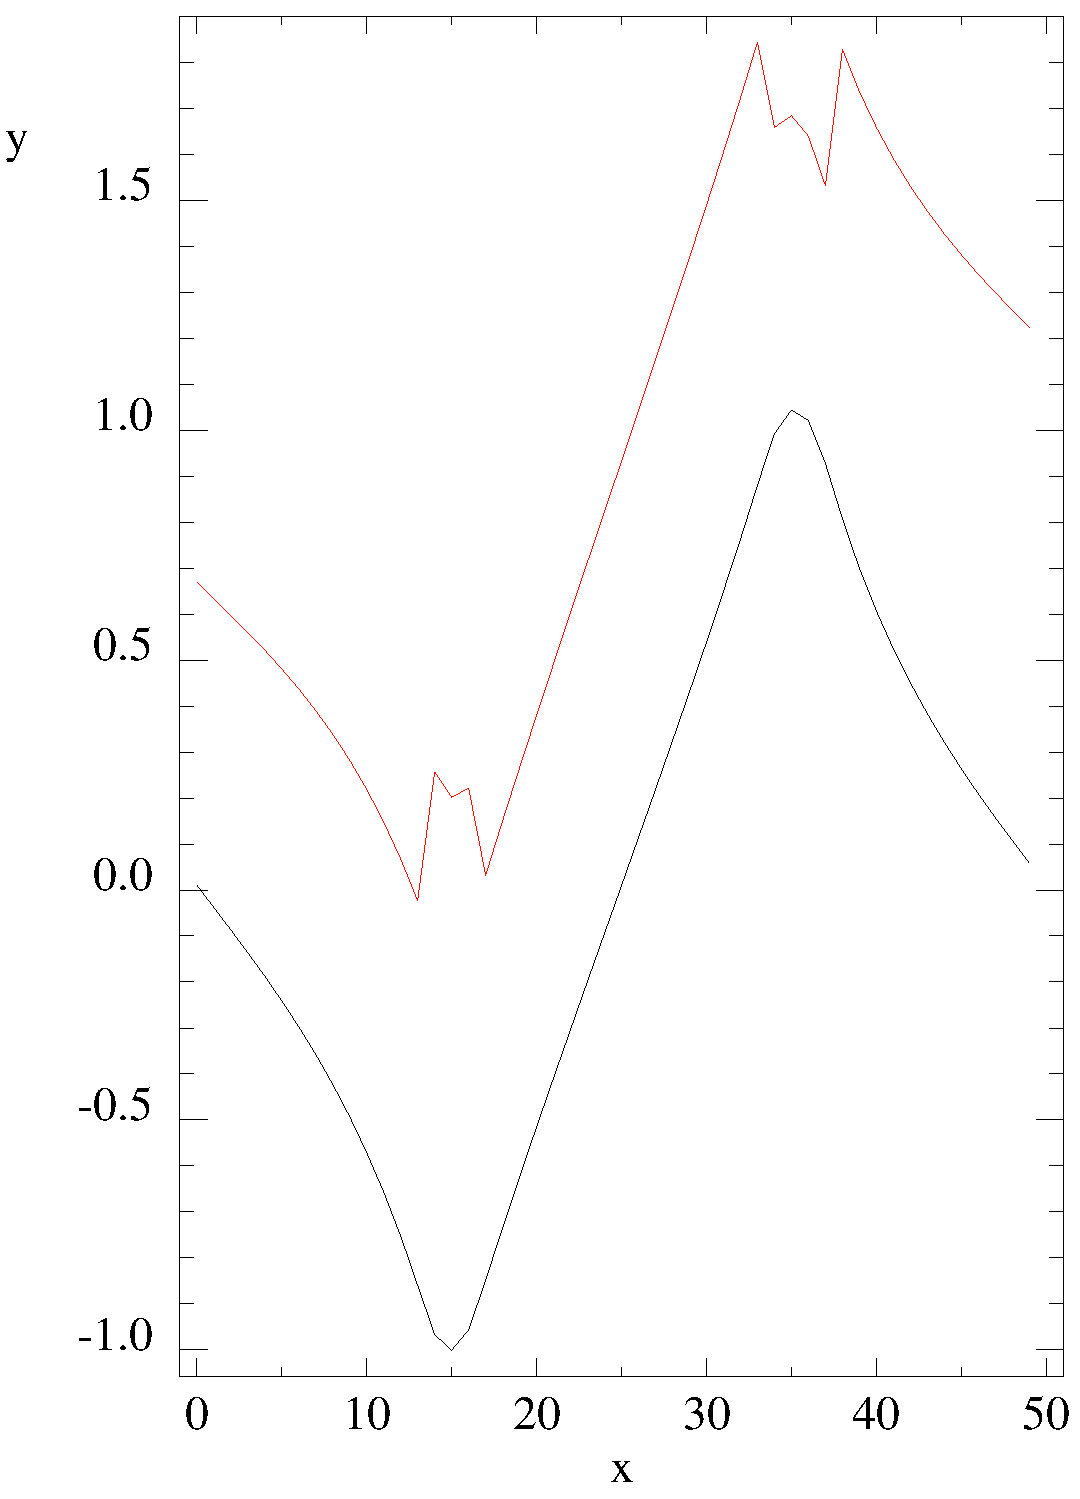
\includegraphics[scale=.7]{Simulations/Analytical-Sim.eps} 

Above is a cross sectional slice of the center of the coil of the magnetic vector potential. The red line is the analytical solution and the black line is the model solution. The discontinuities at the tips of the red line are the areas where current is flowing, and are skipped in the calculation since they represent a division by zero. This doesn't contribute to the B field in the area of interest, so the effects are negligible. Additionally one notes the lines are offset, but since the curl is a derivative operation, the offset doesn't matter since only the slope of the line contributes to the B field.

\includegraphics[scale=.7]{Simulations/Bfield-Face.eps} 

Here is cross sectional view across the face of the coil, displaying the intensity of the B field. Note how the field is uniform.

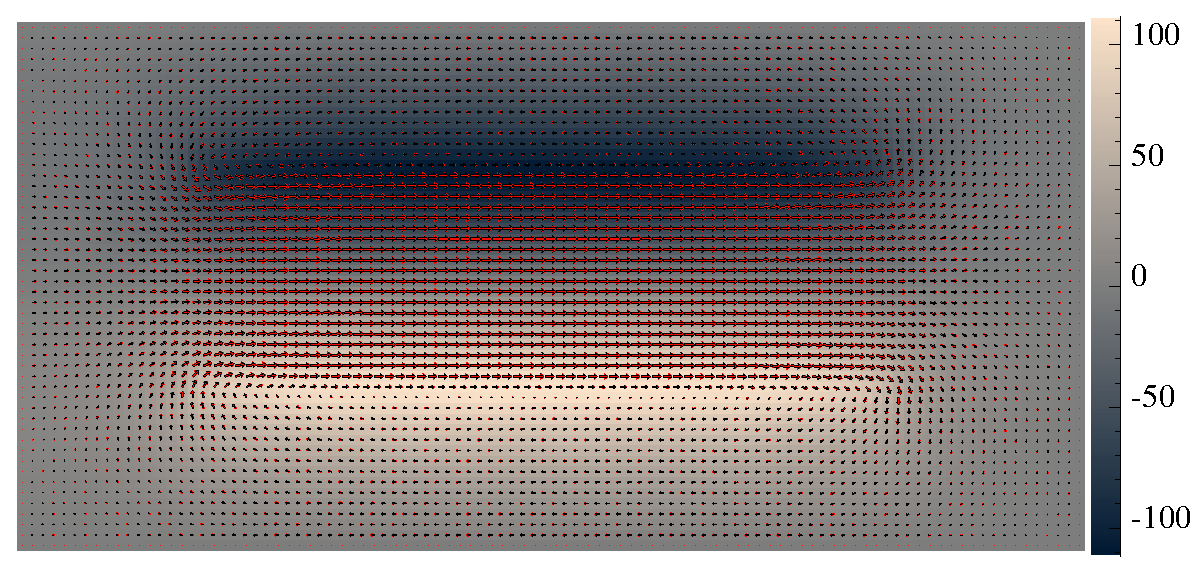
\includegraphics[scale=.7]{Simulations/Coil-and-B-field.eps} 

This length-wise slice shows the B field in vector form. Again, notice how the B field has a uniform direction and intensity, just as expected. 

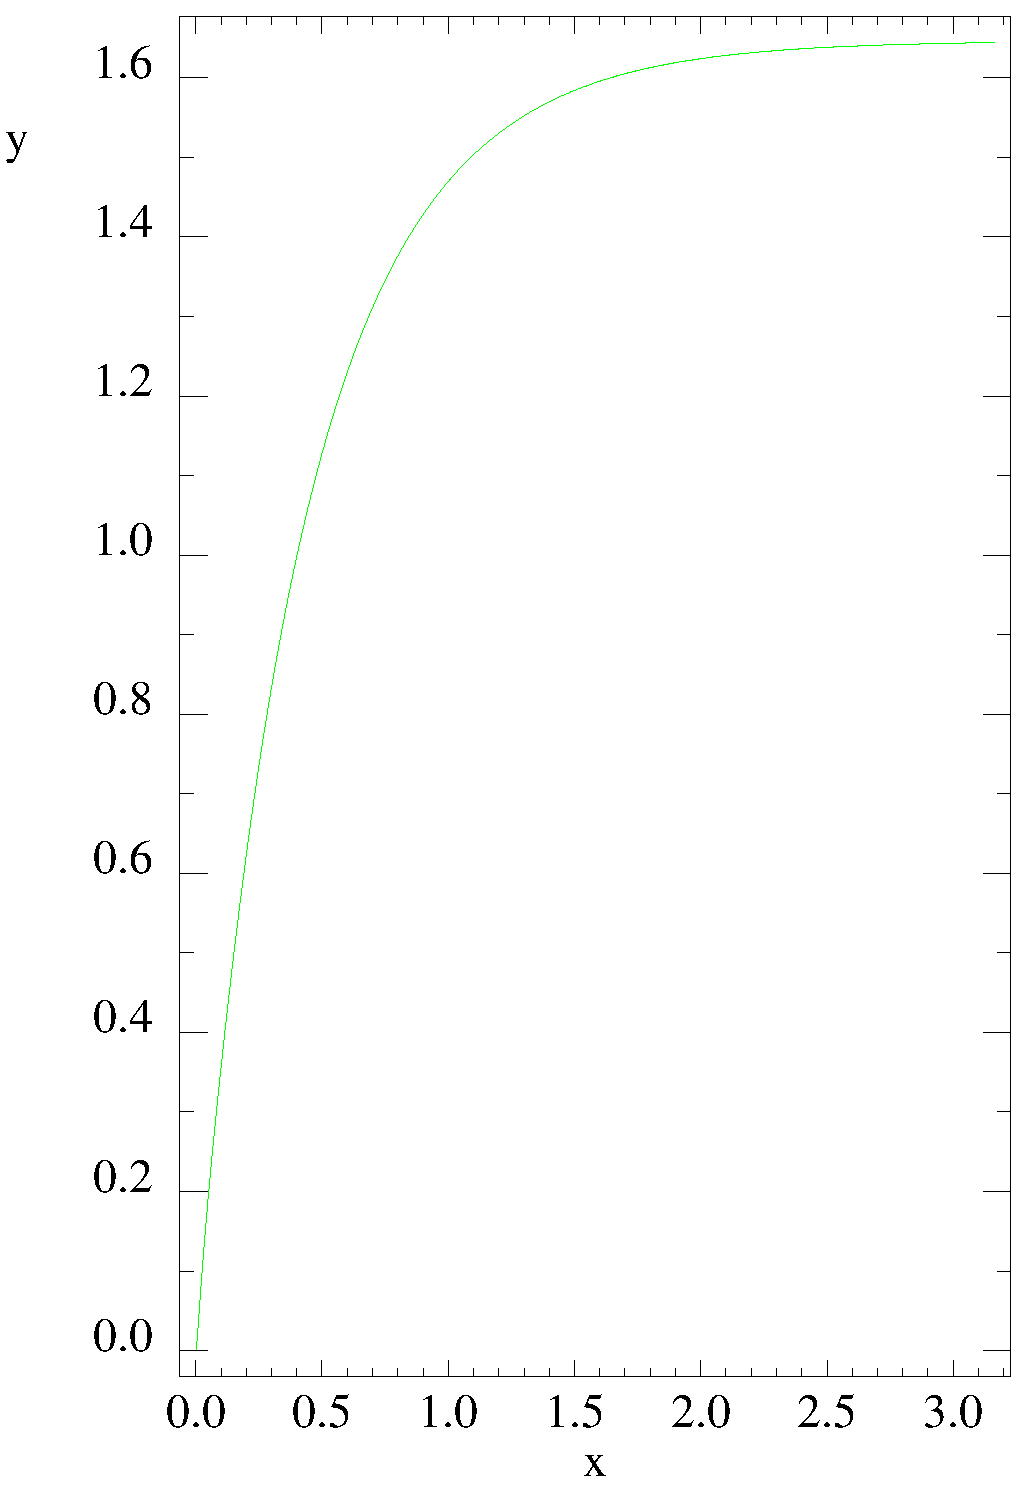
\includegraphics[scale=.7]{Simulations/Energy-Curve.eps} 

One charactaristic inherent from an inductor is the exponential decay behavior that creates hystersis in AC circuits. This appeared in the model as well, dispite the lack of time dependence in the model. 

Much work was put into modeling the behavior of fields that have variable magnetic permeability (a piece of iron). Simulation stability was tedious at best due to extreme values in the mobility, and is an area of further interest.

\section{Ferroic Material Model}

\begin{equation}
-\frac{1}{\mu} \nabla^2 A = J_m 
\end{equation}
\begin{equation}
-\frac{1}{\mu^2} (\partial_v A_\alpha) (\partial_\alpha \mu) = J_{ind}
\end{equation}
\begin{equation}
H = \frac{1}{\mu_0}B - M
\end{equation}


\end{document}